\chapter{Modelagem}

O presente trabalho resolve o problema da maior subsequência comum à 
duas palavras \emph{(LCS)} apresentando três soluções. Cada solução 
engloba um paradigma de programação.

A primeira solução apresenta uma abordagem \emph{força bruta} Ótima. A 
segunda utiliza o paradigma \emph{guloso} e discute a otimalidade da 
solução. A terceira apresenta um algorítmo Ótimo utilizando 
\emph{programação dinâmica} e discorre sobre sua \emph{subestrutura 
ótima} e \emph{sobreposição de subproblemas}, além de apresentar a 
\emph{equação de recorrência} em que o algorítmo é baseado.

\section{Metodologia}

\subsection{Estrutura de diretórios}
jkadjdkljsjskl

\subsection{Como executar os programas}
blabla

\subsection{Documentação}
latex e codigo

\section{Solução}

\subsection{Força Bruta}

Em uma abordagem \emph{força bruta} para resolver o \emph{LCS} deve-se
enumerar todas as subsequências de uma palavra $X$ e verificar se cada
subsequência é comum a outra palavra $Y$. Com isso recuperar a maior 
subsequência comum às duas palavras. 

Dada uma palavra $X$ de tamanho n, tem-se que o número de
subsequência possíveis em $X$ pode ser representado por $2^n$. Essa 
abordagem requer um custo de tempo exponencial para chegar a solução, 
logo, impraticável para sequências muito longas. Para encontrar todas
as combinações (subsequências) foi utilizado um critério de caminhamento
sistemático em uma \emph{árvore de recursão}. Para compreender a 
estratégia, suponha uma palavra $X = abc$ cuja a \emph{árvore de 
recursão} pode ser vista na figura \ref{fig:recursiontree}.

\begin{figure}[H]
    \begin{center}
        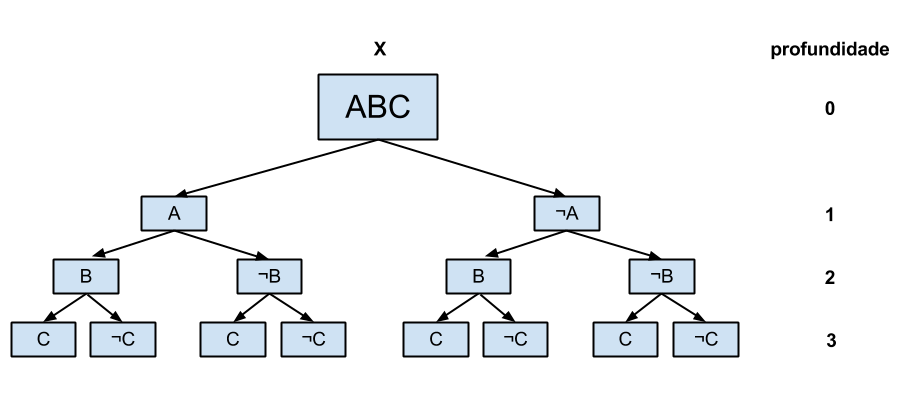
\includegraphics[width=0.8\textwidth,natwidth=610,natheight=642]{doc/recursion-tree.png}
        \caption{Árvore de Recursão}
        \label{fig:recursiontree}
    \end{center}
\end{figure}

A implementação do método \emph{força bruta} é composto por três funções:

\begin{lstlisting}
int brute_force(int k, const char *word0, int sw0, const char *word1, int sw1);
int subsequence(int k, const char* word, const char* other, char* subseq, int n, int seq, int lcs);
int compare(int k, const char* word, const char* subseq);
\end{lstlisting}

A função {\it brute\_force} recebe o tamanho $k$, que representa o 
tamanho mínimo para uma subsequência válida. Recebe também as 
palavras {\it word0} e {\it word1} a serem analisadas assim 
como seus respectivos tamanhos. Essa função é executada para cada $K$
e cada par de palavras lidos do arquivo até que o $K$ lido seja $0$.

{\it subsequence} é uma função recursiva de caminhamento pela 
\emph{árvore de recursão} para encontrar a maior subsequência comum.
São passados $K$, \emph{word0}, \emph{word1} a serem analisados pela
função assim como \emph{subseq} que representa a subsequência 
disponível até o momento, $n$ que é o índice (posição) da subsequência
até o momento, \emph{seq} representando o tamanho da sequencia atual 
para satisfazer a condição \emph{seq} $\ge K$ e \emph{lcs} que é 
a maior subsequencia comum às duas palavras analisadas. 

{\it subsequence} executa duas principais tarefas. Primeiramente 
verifica o caso base ou se o fim da recursão ocorreu. Caso positivo
verifica a ocorrência da atual subsequência da palavra \emph{word0} 
em \emph{word1}:

\begin{lstlisting}
// if is subsequence of the other word
if (compare(k, other, subseq))
    // then, the size of subsequence is as a LCS candidate
    return n;
\end{lstlisting}

A segunda tarefa consiste em executar a chamada recursiva para executar
o caminhamento sistemático pela \emph{árvore de recursão} e encontrar 
as combinações que compõem as subsequências a serem analizadas sempre 
considerando a restrição imposta por $K$.

\begin{lstlisting}
// makes a recursive solution of the left branch
lcs0 = subsequence(k, word + 1, other, subseq, n + 1, seq + 1, lcs);
 .
 .
// makes a recursive solution of the right branch
lcs1 = subsequence(k, word + 1, other, subseq, n, 0, lcs);
\end{lstlisting}

A função \emph{compare} é responsável por verificar a ocorrência de uma 
subsequência de uma palavra em outra palavra. É retornado o tamanho da 
subsequência encontrada ou 0 {\it false} caso contrário.  

\subsubsection{Análise}

A taxa de crescimento de tempo (complexidade de tempo) da função 
\emph{compare} é $T(n) = O(n)$, onde $n$ representa o tamanho da
subsequência a ser encontrada. A complexidade de espaço dessa 
função é T(n) = O(1), logo, constante.

Para compreender a complexidade de tempo e espaço da função 
\emph{subsequence} assume-se:

\begin{math}
$n = $ \textnormal{ tamanho da palavra \emph{word0}} \\
$m = $ \textnormal{ tamanho da palavra \emph{word1}} \\
$T(1) = O(m)$ \textnormal{ considerando a complexidade da função  \emph{compare}} \\ \\
$T(n) = 2T(n - 1) + O(1)$ \\
$T(n) = 2(2(2\dots(T(1) + O(1))\dots + O(1)) + O(1)) + O(1)$ \\
2^{n-1}(O(m) + O(1)) + O(1) \\
2^n(O(m)) \\
O((2^n)*m)
\end{math}

A equação $T(n) = O(n^n*m)$ gera um plano. Para representá-la em um 
gráfico em duas dimensões, suponha $n = m$:

\begin{figure}[H]
    \begin{center}
        \input{doc/gnuplot/brute-time.tex}
        \caption{Complexidade de tempo - Algorítmo Força Bruta}
        \label{fig:brutetime}
    \end{center}
\end{figure}


Temos então que a complexidade de tempo desse algorítmo é custosa
e impraticável para sequências muito grandes. A complexidade de 
espaço é pode ser definida por: 


\begin{math}
T(n) = O(1) \textnormal{ considerando a complexidade em \emph{compare}} \\ \\
T(n) = T(n - 1) + O(1) \\
T(n) = (((T(1) + O(1))\dots) + O(1)) + O(1) \\
T(n) = (((O(1) + O(1))\dots) + O(1)) + O(1) \\
T(n) = n*(O(1)) \\
T(n) = O(n)
\end{math}

O crescimento de espaço desse algorítmo é equivalente ao ramo da árvore 
cuja subsequência é pesquisada. 


\subsection{Guloso}


\subsection{Programação Dinâmica}

A modelagem do problema através da \emph{programação dinâmica} requer 
satisfazer alguns requesitos. O problema deve possuir 
\emph{subestrutura ótima} e \emph{sobreposição de sub-problemas}. 

Para provar a \emph{substrutura ótima} do problema, ele deve consistir 
em fazer escolhas. Essas escolhas deixam um ou mais subproblemas a serem 
resolvidos. O LCS apresenta essa característica em que, a escolha a ser 
feita consiste em encontrar uma subsequência em uma palavra. Ao encontrar,
restam subproblemas de mesma natureza para o resto da palavra ainda não 
pesquisado. 

O problema proposto pelo presente trabalho insere um $K$ que limita o 
tamanho mínimo para os seguimentos que compõem uma subsequência. Então
para um subproblema considere as palavras $X=\{x_1,x_2,x_n\}$, 
$Y=\{y_1,y_2,y_m\}$ e um $K=1$. Considere também que a LCS de $X$ e $Y$ 
é representada por $Z=\{z_1,z_2,z_i\}$. Em função disso, considere $Z$ 
uma \emph{solução ótima} para o problema, então podemos demonstrar que 
feita uma escolha, restam subproblemas a serem resolvidos assim descritos:

\begin{math}
    \textnormal{ se } X_n = Y_m \textnormal{ e } X_n > K
    \textnormal{ então } Z_i = X_n = Y_m
    \textnormal{ e } Z_{i-1} \textnormal{ é LCS de } X_{n-1} 
    \textnormal{ e } Y_{m-1} \\
    \textnormal{ se } X_n \ne Y_m, \textnormal{ então } Z_i \ne X_n 
    \textnormal{ então } Z \textnormal{ é LCS de } X_{n-1} 
    \textnormal{ e } Y \textnormal{ se } X_{n-1} > K \\
    \textnormal{ se } X_n \ne Y_m, \textnormal{ então } Z_i \ne Y_m 
    \textnormal{ então } Z \textnormal{ é LCS de } X 
    \textnormal{ e } Y_{m-1} \textnormal{ se } X_{n-1} > K \\
\end{math}

Se $Z$ é a \emph{solução ótima} então, por contradição, para provar 
a \emph{substrutura ótima} tem-se:

\begin{math}
    SUBSEQ = \textnormal{uma subsequência comum} \\ \\
    Z_i \ne X_n \to Z = SUBSEQ(X_{n-1}, Y) \wedge X_{n-1} > K \\
    \exists W = \{w_1,w_2,w_j\} \; / \; W = SUBSEQ(X_{n-1}, Y) 
    \wedge j > i \\ \therefore W = SUBSEQ(X_n, Y) \to Z \ne LCS(X, Y)
\end{math}

A \emph{sobreposição de subproblemas} define que o espaço de subproblemas
deve ser pequeno. Uma representação recursiva do problema em que a recursão
resolve os mesmos subproblemas repetidas vezes demonstra essa propriedade
em que os os subproblemas são sobrepostos. Ou seja, a solução global 
depende das soluções intermediárias. Observando o problema LCS é nítido
que para encontrar a LCS de duas palavras é necessário resolver as demais
subsequências das palavras para encontrar a LCS. Considerando a modelagem 
apresentada anteriormente para a \emph{programação dinâmica} pode-se definir 
o problema com a seguinte \emph{equação de recorrência}:

\begin{math}
    c[i,j] = \textnormal{comprimento da LCS de um subproblema em} 
    X_i \textnormal{ e } Y_i \\
    K = \textnormal{ tamanho mínimo de um seguimento } \\ \\
    c[i,j] = \Bigg\{
        \begin{array}{l l}
            0 & \textnormal{ se } i = 0 \vee j = 0 \\
            c[i-1,j-1] + 1 & \textnormal{ se } i \wedge j > 0 \wedge
            X_i = Y_j \wedge X_i > K \\
            max(c[i,j-1], c[i-1,j]) & \textnormal{ se } i \wedge 
            j > 0 \wedge X_i \ne Y_j \wedge X_i > K 
        \end{array}
\end{math}



